\section{ Question 2 }\label{sec:q2}    
\begin{enumerate}[a.]

\item
The asked sketch is given below.
\begin{figure}[H]
\centering
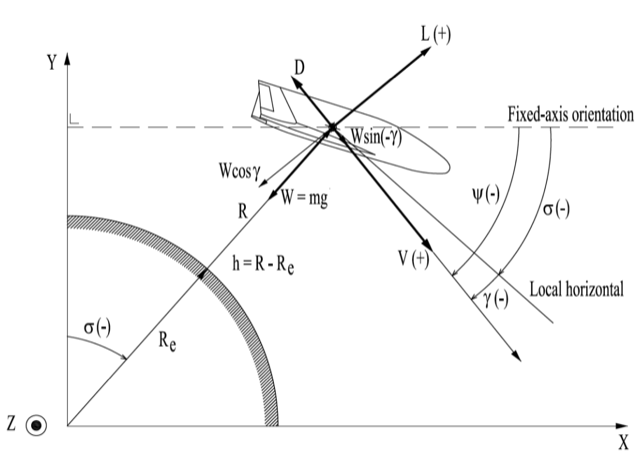
\includegraphics[scale=0.85]{2DPlanarMotion.png}
\end{figure}


\item

\begin{equation}
\(\mathrm{m}\frac{\mathrm{d} \mathrm{V}}{\mathrm{dt}}=-\mathrm{D}-\mathrm{mg} \sin \gamma\)
\end{equation}


\begin{equation}
\(\mathrm{m} \mathrm{V} \frac{\mathrm{d} \gamma}{\mathrm{dt}}=\mathrm{L}-\operatorname{mg} \cos \gamma\left(1-\frac{\mathrm{V}^{2}}{\mathrm{V}_{\mathrm{c}}^{2}}\right)\)
\end{equation}

\begin{equation}
\(\frac{\mathrm{d} \mathrm{R}}{\mathrm{dt}}=\frac{\mathrm{dh}}{\mathrm{dt}}=\mathrm{V} \sin \gamma\)
\end{equation}

The derivation of the EOM's can be found in (reader p.215-219). For the test no derivations are asked for, the equations should be memorized by heart. 

\item
\begin{equation}
\(\mathrm{m} \mathrm{V} \frac{\mathrm{d} \gamma}{\mathrm{dt}}=\mathrm{L}-\operatorname{mg} \cos \gamma\left(1-\frac{\mathrm{V}^{2}}{\mathrm{V}_{\mathrm{c}}^{2}}\right)\)
\label{eq:EOM3}
\end{equation}

By definition of a ballistic flight the lift encountered lift by the vehicle is zero $L=0$. As a consequence the mass can be divided out. We introduce the altitude $h$ as an independent variable, instead of $t$, such that:\\

\begin{equation}
\frac{d \gamma}{d t}=\frac{d \gamma}{d h} \frac{d h}{d t}=V \sin \gamma \frac{d \gamma}{d h}
\label{eq:kinematic}
\end{equation}
Substituting \ref{eq:kinematic} into \ref{eq:EOM3} gives us:

\begin{equation}
\(\mathrm{V}^{2} \sin \gamma \frac{\mathrm{d} \gamma}{\mathrm{dh}}=-\mathrm{g} \cos \gamma\left(1-\frac{\mathrm{V}^{2}}{\mathrm{V}_{\mathrm{c}}^{2}}\right)\)
\end{equation}

\begin{equation}
\(\operatorname{tan} \gamma \frac{\mathrm{d} \gamma}{\mathrm{dh}}=-\mathrm{g}\left(\frac{1}{\mathrm{V}^{2}}-\frac{1}{\mathrm{V}_{\mathrm{c}}^{2}}\right) \approx 0\)
\end{equation}
Assuming $V_c>>V$ and $V^2>>g$ we obtain the following relationship.
\begin{equation}
\(\frac{\mathrm{d} \gamma}{\mathrm{dh}} \approx 0\)
\end{equation}

\begin{equation}
\(\gamma \approx\) constant \(=\gamma_{\mathrm{E}}\)
\end{equation}

Since the Flight Path Angle is constant and does not change w.r.t. height, the trajectory of the ballistics craft is said to be a straight line from entry until it reaches the surface.
\item
This question follows the derivation given in (reader p.262). For a gliding entry we assume that $\frac{\mathrm{d} \gamma}{\mathrm{dt}}=0$ and that the flight path angle $\gamma$ goes to zero.  
\begin{equation}
\(\frac{\mathrm{d} \mathrm{V}}{\mathrm{dt}}=-\frac{\mathrm{D}}{\mathrm{m}}=-\frac{\mathrm{D}}{\mathrm{L}} \mathrm{g}\left(\frac{\mathrm{L}}{\mathrm{mg}}\right)=-\frac{\mathrm{D}}{\mathrm{L}} \mathrm{g}\left(1-\frac{\mathrm{V}^{2}}{\mathrm{V}_{\mathrm{c}}^{2}}\right)\)
\label{eq:DVDT}
\end{equation}

\begin{equation}
\(\mathrm{L}=\mathrm{mg}\left(1-\frac{\mathrm{V}^{2}}{\mathrm{V}_{\mathrm{c}}^{2}}\right)\)
\label{eq:L}
\end{equation}
Now we substitute \ref{eq:L} back into \ref{eq:DVDT} and obtain the following expression for $dt$:

\begin{equation}
\(\mathrm{dt}=-\frac{\frac{\mathrm{L}}{\mathrm{D}}}{\mathrm{g}\left(1-\frac{\mathrm{V}^{2}}{\mathrm{V}_{\mathrm{c}}^{2}}\right)} \mathrm{d} \mathrm{V}\)
\end{equation}

For simplicity means, we substitute $V/V_c=x$ and integrate the expression we found for $dt$ to obtain an expression for the flight time $t_{flight}$

\begin{equation}
\(\mathrm{x}=\frac{\mathrm{V}}{\mathrm{V}_{\mathrm{c}}} ; \mathrm{dx}=\frac{\mathrm{d} \mathrm{V}}{\mathrm{V}_{\mathrm{c}}} \Rightarrow \mathrm{d} \mathrm{V}=\mathrm{V}_{\mathrm{c}} \mathrm{d} \mathrm{x}\)
\end{equation}

\begin{equation}
\(\mathrm{dt}=-\frac{\frac{\mathrm{L}}{\mathrm{D}}}{\mathrm{g}\left(1-\mathrm{x}^{2}\right)} \mathrm{V}_{\mathrm{c}} \mathrm{dx}=-\frac{\mathrm{L}}{\mathrm{D}} \frac{\mathrm{V}_{\mathrm{c}}\left(\frac{\mathrm{dx}}{1-\mathrm{x}^{2}}\right)}{\mathrm{g}}\)
\end{equation}

\begin{equation}
\int(\frac{\mathrm{d} \mathrm{x}}{1-\mathrm{x}^{2}})=\frac{1}{2} \int \frac{\mathrm{dx}}{1+\mathrm{x}}+\frac{1}{2} \int \frac{\mathrm{dx}}{1-\mathrm{x}}=\frac{1}{2} \ln (1+\mathrm{x})-\frac{1}{2} \ln (1-\mathrm{x})+\mathrm{c}=\frac{1}{2} \ln \frac{1+\mathrm{x}}{1-\mathrm{x}}+\mathrm{c}
\end{equation}


\begin{equation}
\(\mathrm{t}_{\text {flight }}=-\frac{\mathrm{V}_{\mathrm{c}}}{\mathrm{g}} \frac{\mathrm{L}}{\mathrm{D}} \int_{\frac{\mathrm{V}_{\mathrm{E}}}{\mathrm{V}}_{\mathrm{C}}}^{\frac{\mathrm{V}_{\mathrm{F}}}{V_{\mathrm{C}}}} \frac{1}{1-\frac{\mathrm{V}_{\mathrm{}}^{2}}{V_c^2}} \mathrm{d}\left(\frac{\mathrm{V}}{\mathrm{V}_{\mathrm{c}}}\right)=-\frac{\mathrm{V}_{\mathrm{c}}}{2 \mathrm{g}} \frac{\mathrm{L}}{\mathrm{D}}\left[\ln \left(\frac{1+\mathrm{V}_{\mathrm{F}} / \mathrm{V}_{\mathrm{c}}}{1+\mathrm{V}_{\mathrm{E}} / \mathrm{V}_{\mathrm{c}}}\right)-\ln \left(\frac{1-\mathrm{V}_{\mathrm{F}} / \mathrm{V}_{\mathrm{c}}}{1-\mathrm{V}_{\mathrm{E}} / \mathrm{V}_{\mathrm{c}}}\right)\right]\)
\end{equation}

\begin{equation}
\mathrm{t}_{\text {flight }}=-\frac{\mathrm{V}_{\mathrm{c}}}{2 \mathrm{g}} \frac{\mathrm{L}}{\mathrm{D}} \ln \left\{\frac{1+\mathrm{V}_{\mathrm{F}} / \mathrm{V}_{\mathrm{c}}}{1-\mathrm{V}_{\mathrm{F}} / \mathrm{V}_{\mathrm{c}}} \cdot \frac{1-\mathrm{V}_{\mathrm{E}} / \mathrm{V}_{\mathrm{c}}}{1+\mathrm{V}_{\mathrm{E}} / \mathrm{V}_{\mathrm{c}}}\right\}
\end{equation}


Assuming $V_F<<V_c$, we obtain the following expression for the flight time. 

\begin{equation}
\(\mathrm{t}_{\text {flight }}=\frac{\mathrm{V}_{\mathrm{c}}}{2 \mathrm{g}} \frac{\mathrm{L}}{\mathrm{D}} \ln \left(\frac{1+\mathrm{V}_{\mathrm{E}} / \mathrm{V}_{\mathrm{c}}}{1-\mathrm{V}_{\mathrm{E}} / \mathrm{V}_{\mathrm{c}}}\right)\)
\end{equation}

\item
Filling in the numbers gives us, 
\begin{equation}
\(\mathrm{t}_{\text {flight }}=\frac{7920}{2 \mathrm{9.81}} *(-2)* \ln \left(\frac{1+0.8}{1-0.8}\right)\)
\end{equation}

\begin{equation}
\mathrm{t}_{\text {flight }}=1773.9s 
\end{equation}










\end{enumerate}